\chapter*{Problema I - Inverosímil}

\begin{center}
  \begin{tabular}{ | l | l | l | }
    \hline
    Tiepo Límite: 2u & Memoria Límite: 512mb & Código Fuente: \texttt{inverosimil.\{java|cpp|c|py\}} \\
    \hline
  \end{tabular}
\end{center}

 .\\
-Es verosímil la cantidad de estrellas en el firmamento \\
-Es inverosímil que ...

Mientras Paquita Cabeza y El Mai platicaban sobre cosas que van más allá del entendimiento humano, llegó a su mente la siguiente pregunta: ¿Cuánto paralelogramos puedes formar con $n$ lineas paralelas que se intersectan con otras $m$ lineas paralelas
\subsection*{}
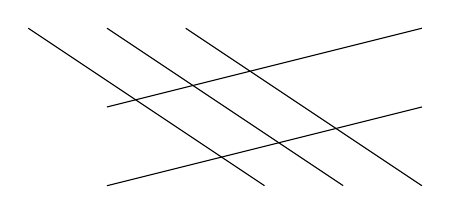
\begin{tikzpicture}

\draw (0,0) -- (4,1);
\draw (0,1) -- (4,2);
\draw (2,0) -- (-1,2);
\draw (3,0) -- (0,2);
\draw (4,0) -- (1,2);

\end{tikzpicture}\\
$2$ lineas paralelas se intersectan con otras $3$ lineas paralelas
\subsection*{Entrada}

La primera línea de entrada será un número $C$ $(1 \leq  C\leq 1000)$, que es el número de casos de prueba, después vendrán $C$ casos. Cada caso tiene una linea con dos números $n$ y $m$, que indican que hay $n$ lineas paralelas que se intersectan con otras $m$ lineas paralelas

\subsection*{Salida}
Para cada caso indica la cantidad de paralelogramos que se pueden formar.

\subsection*{Limites de los conjuntos de datos}
\begin{itemize}
    \item Pequeño: $ 2\leq n,m \leq 10  $ $\quad \quad \quad$ $35$ puntos.
    \item Mediano: $ 2\leq n,m \leq 100  $ $\quad \quad \;$ $35$ puntos.
    \item Grande: $ 2\leq n,m \leq 10000  $ $\quad \quad$ $30$ puntos.
\end{itemize}

\begin{multicols}{2}
\subsection*{Entrada Ejemplo}
\begin{verbatim}
2
2 2
2 3
\end{verbatim}
\columnbreak
\subsection*{Salida Ejemplo}
\begin{verbatim}
1
3
\end{verbatim}
\end{multicols}
